%
% Anlagendesign
%
% @version 1.0
% @author dmayer
% @created 29. Dezember 2015

\setchapterpreamble[o]{%
\dictum[--- \textsc{Norbert Wiener}]{\Gun Das beste Modell für eine Katze ist eine Katze; möglichst dieselbe Katze. \Gob}}
\renewcommand{\chapterheadstartvskip}{\vspace*{2cm}}

\chapter{Modellbildung des Raumes}
\label{chap:modellbildung}

\lstinputlisting[language=Modelica, linerange=194-20, label=lst:room]{listings/room_model_listing.mo}

Ziel dieses Kapitels ist es, ein hinreichend exaktes Modell zur Berechnung der Raumtemperatur, basierend auf den thermodynamischen Prozessen mit dessen Umgebung und der Anlage aus Kapitel \ref{chap:anlagendesign}, zu bilden, um damit und unter Zuhilfenahme der Anlage Modellpräditive Regelung zu ermöglichen.
Dazu wird zunächst ein einfaches Grundmodell für einen hypothetischen Raum gebildet, dass anschließend schrittweise an den bestehenden Raum erweitert angepasst wird, bis eine die Qualität des Modells ausreichend ist.

\section{Anforderungen an das Raummodell}
Da MPC die Lösung von Nichtlinearen Gleichungssystemen erfordert wird ein erhöhter Rechenbedarf benötigt. Daher sollte das Modell so einfach wie möglich gehalten werden. Die Krux liegt also darin, einen geeigneten Kompromiss zwischen Komplexität und Genauigkeit des Modells zu finden, der eine sinnvolle MPC Regelung ermöglicht.
Des Weiteren werden gradientenbasierte Ableitungen bei der Optmierung/Lösung des LGS generiert weshalb auch keine Unstetigkeiten im Modell vorkommen dürfen.
Die triviale Aufgabe ist die hinreichend genaue Beschreibung der Realität bzw realen Vorgänge.
Damit eine Steuerung mit Hilfe von Modellprädiktiver Regelung möglich ist, darf das Modell keine hohe Kompliziertheit aufweisen und sollte durch möglichst wenig Gleichunge trotzdem ein möglichst genaues Abbild der Realität abbilden.
Das Modell soll zunächst so simpel wie möglich gestaltet werden um eine Optimierung mit Hilfe von MPC zu ermöglichen. Dessen Verfahren zur Optimierung sind gradientenbasiert und erfordern damit die Erzeugung von stetigen Ableitungen bis zum zweiten Grad. Daher soll die Komlpexität des Modells zunöchgst sehr gering gehalten werdeen und dann Stück für Stück erhöht werden und die damit die Geanuiogkeit des modells erhöht werden

\section{Das Grundmodell des Raumes}

Um ein möglichst einfaches Grundmodell zu erhalten, wird zunächst ein hypothetischer Raum betrachtet. Dieser Raum bildet zusammen mit der ihn umgebenden Luft ein abgeschlossenes thermodynamisches System, wie in Kapitel \ref{sec:grundlagenmodell} beschrieben. Der Raum ist selbst mit Luft gefüllt und wird zu allen sechs Seiten hin durch Wände begrenzt. Damit bildet der Raum ein geschlossenes System, da keine Massenströme über die Grenzen hinweg fließen können. An den Grenzflächen kann also lediglich Wärme zwischen der Luft außerhalb und innerhalb des Raumes ausgetauscht werden. Des Weiteren wird eine homogene Temperatur innerhalb des Raumes und der Umgebung angenommen, was einem eingeschwungenen Zustand/Gleichgewichtszustand in der Realität entspricht. Diese Annahme ist jedoch noch zu überprüfen.

\begin{figure}
\centering
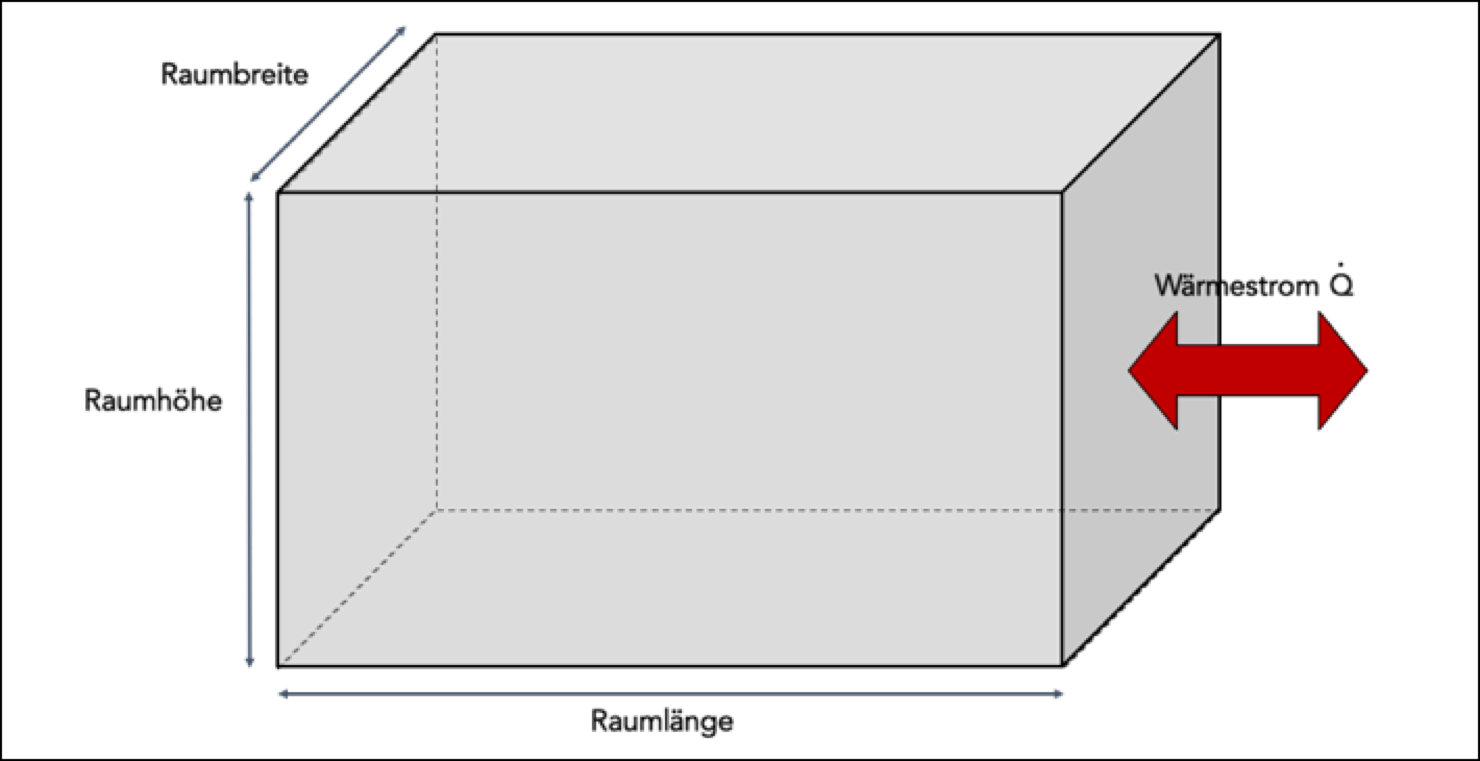
\includegraphics[width=\textwidth]{abbildungen/20160316_grundraum}
\caption{Grundmodell eines Raumes}
\label{fig:grundraum}
\end{figure}

Zur Bestimmung der Raumtemperatur muss, ausgehend von einer initialen Raumtemperatur und der Umgebungstemperatur, der Ausgleichsprozess zwischen Raum und Umgebung untersucht werden, konkret der ausgetauschte Wärmestrom. Um diesen nach \ref{eq:qdot} zu berechnen, müssen zunächst die verschiedene modellrelevanten Eigenschaften des Raumes durch physikalische Größen und Variablen beschrieben werden. Zur Berechnung der Austauschoberfläche wird die Raumbreite, -länge und -höhe benötigt und weiterhin sind der U-Wert einer Betonwand, die spezifische Wärmekapazität und Dichte von Luft für die Bestimmung des Wärmestroms relevant.

Diese modellrelevanten Eigenschaften sind allesamt mit ihren Zahlenwerten in Tabelle \ref{tab:eigenschaften_raum} zusammengefasst.

\begin{table}[H]
\centering
\small
\renewcommand{\arraystretch}{1.3}
\begin{threeparttable}
\begin{tabularx}{1\textwidth}{p{0.5\textwidth}m{0.2\textwidth}m{0.18\textwidth}}
\toprule
\textbf{Modellrelevante Eigenschaften} & \textbf{Wert} & \textbf{Einheit} \\
\cmidrule[0.5pt](r{0.25em}){1-1} 
\cmidrule[0.5pt](l{0.25em}){2-2}
\cmidrule[0.5pt](l{0.25em}){3-3}

Raumbreite & 7,81\tnote{1)} & $[m]$ \\ 
\ccol Raumlänge & \ccol 5,78\tnote{1)} & \ccol $[m]$ \\
Raumhöhe & 2,99\tnote{1)} & $[m]$ \\
\ccol Wärmedurchgangskoeffizient & \ccol 2\tnote{2)} & \ccol $[\frac{W}{m^{2}*K}]$\\
Spezifische Wärmekapazität von Luft & 1.000\tnote{3)} & $[\frac{J}{kg*K}]$\\
\ccol Dichte von Luft & \ccol 1,25 \tnote{3)} & \ccol $[\frac{kg}{m^{3}}]$\\
\bottomrule
\end{tabularx}
\begin{tablenotes}[]\footnotesize\singlespacing\setlength\labelsep{0pt}
\item[1)] Werte durch eigene Vermessung des Raumes K004b vom 07.12.2015
\item[2)] Schätzwert, geschätzt nach \cite[S.~409]{re14} mit Richtwerten aus \cite[S.~194ff.]{re14}
\item[3)] Tabellenwert aus \cite[S.~139]{ha13}
\end{tablenotes}
\end{threeparttable}
\caption{Eigenschaften des Raummodells}
\label{tab:eigenschaften_raum}
\end{table}

Erfolgt nun die Bilanzierung des Raumes mit Hilfe des ersten Hauptsatzes der Thermodynamik nach \ref{eq:hauptsatz} und die Berechnung der inneren Energie des Raumes nach \ref{eq:innereenergie} ergibt sich folgendes, einfaches Gleichungssystem zur Bestimmung der Raumtemperatur im Grundmodell in Modelica:

\begin{lstlisting}[language=Modelica, label=lst:grundraum]
equation
   /* calculate room volume */
   room_volume = room_length * room_height * room_breadth;
   /* calculate room mass */
   room_mass = room_volume * rho_air;
   /* calculate surface of heat exchange */
   exchange_surface = 2 * (room_length * room_breadth) + 2 * (room_length * room_height) + 2 * (room_breadth * room_height);
   /* calculate inner energy*/
   room_u = room_mass * cp_air * room_temperature;
   /* calculate derivative of the inner energy */
   der(room_u) = environment_qdot;
   /* calculate heatflow between room and environment */
   environment_qdot = u_wall * exchange_surface * (environment_temperature - room_temperature);
\end{lstlisting}

Dieses ist das Grundmodell für einen Raum ist in \ref{fig:grundraum} graphisch dargestellt und wird im Folgenden schrittweise erweitert, um der Realität genüge zu tragen.

\section{Modellerweiterung durch Berücksichtigung der realen Umgebung}

Im nächsten Schritt wird das Raummodell an die reale Umgebung des Raums K004b angepasst. In der \ref{fig:skizzek004a} wird deutlich, dass der Raum lediglich zwei Außenwände besitzt, die an die Umgebungsluft grenzen: Die Wände in Richtung Süden und Westen. Die anderen beiden Wände, sowie die Decke und der Boden, grenzen an weitere Gebäudeteile des K-Gebäudes. Der Raum ist nach wie vor ein geschlossenes System und bildet zusammen mit dem umgebenden K-Gebäude und der Umgebung wiederum ein abgeschlossenes System. Jedoch können nun verschiedene Wärmeströme zwischen dem Raum und der Außenumgebung sowie dem Raum und dem K-Gebäude ausgetauscht werden. Aufgrund der Relation der Wärmeströme im Gegensatz zur großen Energie des K-Gebäudes und der Umgebung, wird der Erwärmungs- bzw Abkühlungseffekt durch den Wärmestrom mit dem Raum vernachlässigt und von konstanten, homogenen Temperaturen innerhalb der Umgebung und des K-Gebäudes ausgegangen.

Durch diese Erweiterung des Modells wird die gesamte Austauschoberfläche zum Wärmeaustauschs aufgeteilt in die Austauschoberfläche mit der Umgebung und die Austauschoberfläche mit dem K-Gebäude, um die Wärmeströme separat berechnen zu können. Des Weiteren werden im Modell die Temperatur der Außenumgebung und die Temperatur innerhalb des K-Gebäudes als externe Steuergrößen berücksichtigt. Das Gleichungssystem des Grundmodells in \ref{lst:grundraum} erweitert sich also um folgende Änderungen:

\begin{lstlisting}[language=Modelica,label=lst:raumeins]
equation
   [...]
   /* calculate surface of heat exchange with environment */
   environment_exchange_surface = room_length * room_height + room_breadth * room_height;
   /* calculate surface of heat exchange with the remaining building */
   building_exchange_surface = 2 * (room_length * room_breadth) + room_length * room_height + room_breadth * room_height;
   /* calculate derivative of the inner energy */
   der(room_u) = environment_qdot + building_qdot;
   /* calculate heatflow between room and environment */
   environment_qdot = u_wall * environment_exchange_surface * (environment_temperature - room_temperature);
   /* calculate heatflow between room and building */
   building_qdot = u_wall * building_exchange_surface * (building_temperature - room_temperature);
\end{lstlisting}

Damit wurde er Raum an die reale Umgebung angepasst und im nächsten Schritt werden die räumlichen Gegebenheiten im Modell abgebildet.

\section{Modellerweiterung durch Berücksichtigung der räumlichen Gegebenheiten}

Das Modell wird nun an die realen Gegebenheiten des Raumes K004b angepasst, welche in \ref{fig:skizzek004a} bereits dargestellt wurden. Zum einen ist in der südlichen Außenwand eine Fensterfront vorhanden und zum anderen ein Heizkörper innerhalb des Raumes vorhanden. Da der U-Wert von Glas erheblich von dem Wert einer Wand abweicht, entsteht ein weiterer Wärmestrom durch die Fenster mit der Umgebungsluft. Des weiteren muss im Modell eine Wärmequelle hinzugefügt werden, um den vom Heizkörper eingebrachten Wärmestrom zu berücksichtigen. Graphisch sind diese Erweiterungen des Modells in \ref{fig:raumeins} zu sehen.

%Here We GO with model extension

\ref{lst:room}

\begin{figure}
\centering
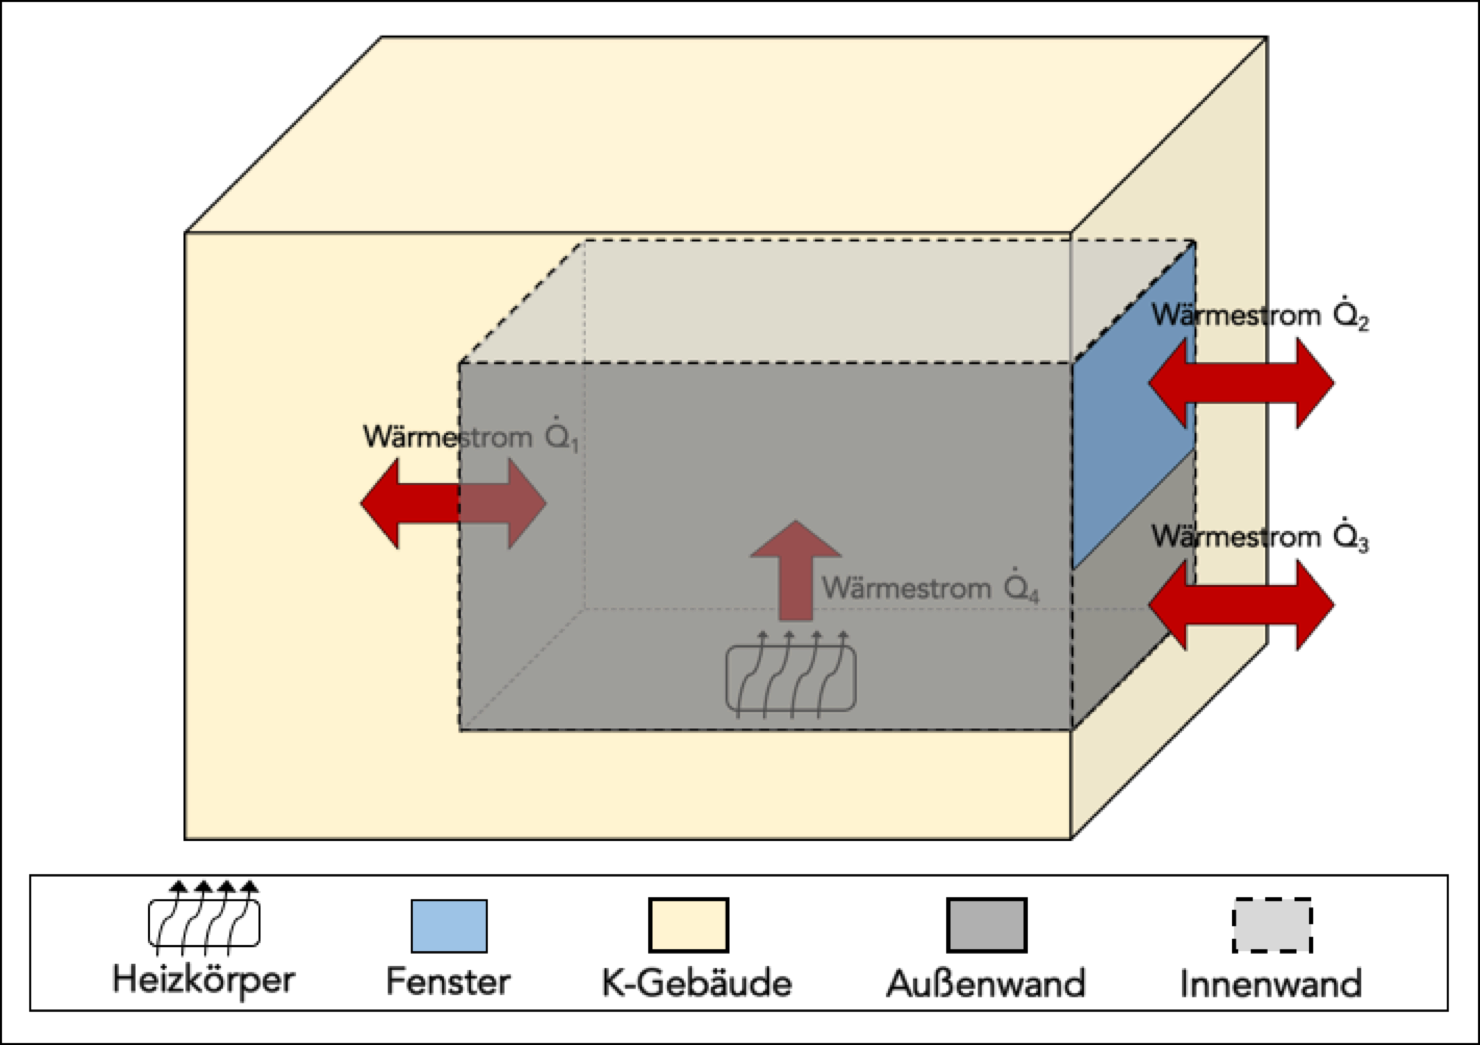
\includegraphics[width=\textwidth]{abbildungen/20160316_raumeins}
\caption{Erweitertes Raummodell}
\label{fig:raumeins}
\end{figure}



\section{Erweiterung durch Sonneneinstrahlung}

\section{Validierung des Modells}

\section{Anpassung des Modells mit Parameterschätzung}